\documentclass[aspectratio=169,10pt]{beamer}
\usetheme{default}

% Exclude appendix slides from the main slide-number count (main shows N/13,
% appendix shows A-1/A-4).
\setbeamertemplate{page number in head/foot}[appendixframenumber]

\usepackage{fontspec}
\setmainfont{TeX Gyre Heros}
\setsansfont{TeX Gyre Heros}
\usepackage{booktabs}
\usepackage{graphicx}
\usepackage{qrcode}
\usepackage{amsmath}
\usepackage{amssymb}
\usepackage{graphicx}
\usepackage{tikz}
\usetikzlibrary{shapes,arrows,arrows.meta,calc,math,positioning}

% ============================================================
%  CUSTOM THEME — "Forensic Navy"
% ============================================================
\definecolor{navy}{HTML}{163A5C}
\definecolor{navylight}{HTML}{2E6199}
\definecolor{navypale}{HTML}{EDF2F7}
\definecolor{amber}{HTML}{D98424}
\definecolor{amberpale}{HTML}{FBEEDD}
\definecolor{teal}{HTML}{0E7C7B}
\definecolor{tealpale}{HTML}{DFF0EE}
\definecolor{slate}{HTML}{5B6472}
\definecolor{inktext}{HTML}{22282E}

\setbeamertemplate{navigation symbols}{}
\setbeamertemplate{itemize item}{\small\raisebox{0.15ex}{\textcolor{amber}{$\blacktriangleright$}}}
\setbeamertemplate{itemize subitem}{\footnotesize\textcolor{navylight}{$\bullet$}}
\setbeamertemplate{enumerate item}{\color{navy}\bfseries\insertenumlabel.}
\setbeamertemplate{caption}[numbered]

\setbeamercolor{normal text}{fg=inktext}
\setbeamercolor{structure}{fg=navy}
\setbeamercolor{alerted text}{fg=amber!85!black}
\setbeamercolor{palette primary}{bg=navy,fg=white}

\setbeamercolor{title}{fg=navy}
\setbeamercolor{subtitle}{fg=slate}
\setbeamercolor{author}{fg=inktext}
\setbeamercolor{institute}{fg=slate}
\setbeamercolor{date}{fg=navylight}

\setbeamercolor{frametitle}{bg=navy,fg=white}
\setbeamerfont{frametitle}{series=\bfseries,size=\large}
\setbeamerfont{framesubtitle}{series=\mdseries,size=\scriptsize}

\setbeamercolor{block title}{bg=navypale,fg=navy}
\setbeamercolor{block body}{bg=navypale!45,fg=inktext}
\setbeamerfont{block title}{series=\bfseries}
\setbeamercolor{block title alerted}{bg=amberpale,fg=amber!70!black}
\setbeamercolor{block body alerted}{bg=amberpale!55,fg=inktext}
\setbeamerfont{block title alerted}{series=\bfseries}

\setbeamercolor{footline}{fg=slate}
\setbeamerfont{footline}{size=\scriptsize}

% Content margins match the slide-title margins (title text starts after the
% 0.13cm amber tab + 0.4cm gap = 0.53cm; title rightskip is 0.55cm).
\setbeamersize{text margin left=0.53cm,text margin right=0.55cm}

% -- frame title: navy band with full-height amber tab --
% Band height/depth are fixed so the amber tab spans the WHOLE band (no stub).
\newlength{\ftbaht}\setlength{\ftbaht}{13pt}
\newlength{\ftbadp}\setlength{\ftbadp}{5pt}
\setbeamertemplate{frametitle}{%
  \nointerlineskip
  \begin{beamercolorbox}[wd=\paperwidth,ht=\ftbaht,dp=\ftbadp,leftskip=0pt,rightskip=0.55cm]{frametitle}%
    {\color{amber}\vrule width 0.13cm height \ftbaht depth \ftbadp}%
    \hspace{0.4cm}\usebeamerfont{frametitle}\insertframetitle%
  \end{beamercolorbox}%
}

% -- footline: page count right only --
\setbeamertemplate{footline}{%
  \begin{beamercolorbox}[wd=\paperwidth,ht=2.0ex,dp=0.9ex,leftskip=0.53cm,rightskip=0.55cm]{footline}%
    \usebeamerfont{footline}\hfill\usebeamertemplate*{page number in head/foot}%
  \end{beamercolorbox}%
}

% -- title page: institution logos, clean centred block --
\setbeamertemplate{title page}{%
  \vspace*{0.4cm}
  \begin{center}
    \begin{tabular}{@{}c@{\hspace{0.6cm}}c@{\hspace{0.6cm}}c@{}}
      \raisebox{0pt}[0pt][0pt]{
\includegraphics[height=1.05cm,keepaspectratio]{Logos/univaq.png}} &
      \raisebox{0.0ex}{
\includegraphics[height=0.84cm,keepaspectratio]{Logos/mathmods.jpg}} &
      \raisebox{0pt}[0pt][0pt]{
\includegraphics[height=1.05cm,keepaspectratio]{Logos/uhh.jpg}}
    \end{tabular}

    \vskip0.28cm
    {\color{navy!70}\rule{\linewidth}{0.8pt}}

    \vskip0.45cm
    {\usebeamercolor[fg]{title}\fontsize{20}{24}\selectfont\textbf{\inserttitle}\par}
    \vskip0.12cm
    {\usebeamercolor[fg]{subtitle}\fontsize{13}{16.5}\selectfont\insertsubtitle\par}

    \vskip0.5cm
    {\fontsize{16}{20}\selectfont\bfseries\color{navy}\insertauthor\par}
    \vskip0.16cm
    {\normalcolor\usebeamercolor[fg]{institute}\insertinstitute\par}
  \end{center}
  \vfill
  {\hfill\small\usebeamercolor[fg]{date}\insertdate\hfill}
  \vskip0.12cm
}

\tikzstyle{interval}            = [line width = 1pt, > = {Circle[length = 3.4pt]}, shorten > = -0pt]
\tikzstyle{interval label}      = [font = {\footnotesize}]

\newcommand*{\Interval}[5][]{%
    \draw[interval, #1] (#2, #4) -- (#3, #4);
    \node[interval label] at (-0.5,#4) {#5};
}

\newcommand*{\RSIntervals}[6]{%
    \Interval[#1]{#2}{#3}{1}{$r$}
    \Interval[#4]{#5}{#6}{0}{$s$}
}

\newcommand*{\DoodleSP}{%
    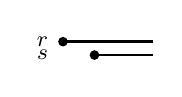
\begin{tikzpicture}[xscale=0.4, yscale=0.17, baseline={($(current bounding box.north)-(0,7.5pt)$)}]
        \RSIntervals{<-}{0}{3}{<-}{1}{3}
    \end{tikzpicture}%
}

\newcommand*{\DoodleBef}{%
    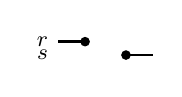
\begin{tikzpicture}[xscale=0.4, yscale=0.17, baseline={($(current bounding box.north)-(0,7.5pt)$)}]
        \RSIntervals{->}{0}{1}{<-}{2}{3}
    \end{tikzpicture}%
}

\newcommand*{\DoodleLOJ}{%
    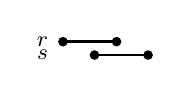
\begin{tikzpicture}[xscale=0.4, yscale=0.17, baseline={($(current bounding box.north)-(0,7.5pt)$)}]
        \RSIntervals{<->}{0}{2}{<->}{1}{3}
    \end{tikzpicture}%
}

\newcommand*{\DoodleDJ}{%
    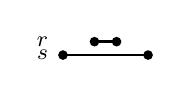
\begin{tikzpicture}[xscale=0.4, yscale=0.17, baseline={($(current bounding box.north)-(0,7.5pt)$)}]
        \RSIntervals{<->}{1}{2}{<->}{0}{3}
    \end{tikzpicture}%
}

\newcommand*{\DoodleEF}{%
    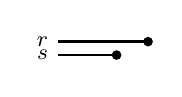
\begin{tikzpicture}[xscale=0.4, yscale=0.17, baseline={($(current bounding box.north)-(0,7.5pt)$)}]
        \RSIntervals{->}{0}{3}{->}{0}{2}
    \end{tikzpicture}%
}

% --- ISEQL temporal operators
\newcommand*{\Bef}{\mathrm{Bef}}
\newcommand*{\SP}{\mathrm{SP}}
\newcommand*{\LOJ}{\mathrm{LOJ}}
\newcommand*{\DJoin}{\mathrm{DJ}}
\newcommand*{\EF}{\mathrm{EF}}
\newcommand*{\size}{\mathrm{size}}

\title[WATCHOUT ISEQL]{WATCHOUT ISEQL}
\subtitle{Large Audio-Language Models and Object Re-Identification\\for Forensic Multimodal Surveillance Event Detection}
\author[G. Rifqialdi]{Ghiffary Rifqialdi}
\institute[Universities]{%
  {\footnotesize Joint Degree of Master of Science in Mathematical Modelling in Engineering: Theory, Numerics, Applications}\\[0.1em]
  {\footnotesize Universit\`a degli Studi dell'Aquila and Universit\"at Hamburg}\\[0.15em]
  {\footnotesize Supervisor: Prof.\ Fabio Persia}\\[0.15em]
  {\scriptsize\itshape\color{slate} Submitted for peer review at the IEEE/CVF WACV 2027, as first author}
}
\date{Master's Thesis Defense}

\begin{document}

\frame{\titlepage}

% ── MOTIVATION ──
\section{Motivation}
\begin{frame}{The Surveillance Problem}
\begin{columns}[c,onlytextwidth]
\column{0.52\textwidth}
Surveillance footage is generated at a \textbf{scale far beyond} human monitoring capacity.\\
\vspace{0.4em}
A human operator watching \textbf{multiple feeds} experiences \alert{vigilance decrement} after approximately 20 minutes.\\
\vspace{0.4em}
Critical events go unnoticed. A missed event could mean a missed crime.

\column{0.48\textwidth}
\begin{block}{Three challenges}
\begin{enumerate}
  \item Visual events need \textbf{cross-frame tracking} to form temporal intervals
  \item Audio captures \textbf{off-camera} events invisible to cameras
  \item Combining modalities naively (temporal joins) \textbf{reduces recall}
\end{enumerate}
\end{block}
\end{columns}
\end{frame}

% ── PROBLEM & GAP ──
\section{Problem and Gap}
\begin{frame}{Prior Work: VIS MODE and Its Limitations}
\footnotesize
\begin{block}{VIS MODE (Crescitelli et al., ECCV 2026)}
First ISEQL-based event detector using VLM perception.
\end{block}
\vspace{0.3em}
\begin{alertblock}{Three problems identified}
\begin{enumerate}
  \item \textbf{Missing re-identification:} VLM assigned new IDs every frame, intervals never spanned multiple frames, \alert{tracking-dependent events undetected}.
  \item \textbf{Unverifiable claims:} Evaluated on unlabeled ground truth.
  \item \textbf{Non-deterministic:} Temperature $>0$, no fixed seed. The model writes descriptions creatively, so results are \alert{not reproducible}: fresh person/object IDs every call mean \alert{handoff failed completely}, because handoff requires the object carried by person A to match the object carried by person B (VIS MODE: 0 detections).
\end{enumerate}
\end{alertblock}
\vspace{0.3em}
\textbf{Our fix:} Object re-identification unlocks tracking-dependent events; temperature $=0$, seed $=42$ make inference deterministic (audio uses greedy decoding, same seed).\hspace{0.5em}\textbf{Our extension:} Audio modality via LALM.
\end{frame}

% ── RESEARCH QUESTIONS ──
\section{Research Questions}
\begin{frame}{Research Questions}
\begin{enumerate}
  \item \textbf{RQ1 (Object Re-Identification)}\\
  How does per-frame object re-identification using a retrieval-augmented object memory affect visual intervals and detected events, compared to no re-identification?
  \vspace{0.4em}

  \item \textbf{RQ2 (Audio Ablation)}\\
  How do Qwen2-Audio-7B-Instruct (LALM) and PANNs CNN14 compare across sliding window and hop configurations on audio-relevant scenes?
  \vspace{0.4em}

  \item \textbf{RQ3 (Multimodal vs.\ Unimodal)}\\
  What is the F1 of visual-only (A), audio-only (B), and multimodal union (C) across all 30 scenes, and does $C \ge \max(A,B)$ hold on every scene?
\end{enumerate}
\end{frame}

% ── SYSTEM OVERVIEW ──
\section{System}
\begin{frame}{What We Built}
\centering
\footnotesize
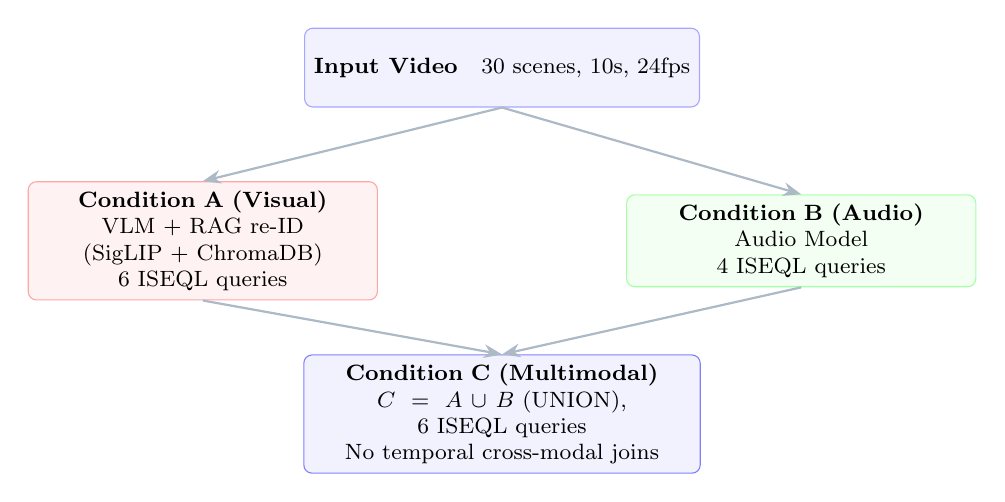
\begin{tikzpicture}[
  node distance=0.6cm,
  box/.style={rectangle,draw=navy!60,fill=navypale,rounded corners=3pt,align=center,minimum height=1.0cm,font=\footnotesize},
  arrow/.style={-Stealth,thick,navy!35},
]
\node[box,fill=blue!5,draw=blue!35] (video) at (0,0) {\textbf{Input Video}\quad 30 scenes, 10s, 24fps};
\node[box,fill=red!5,draw=red!35,text width=4.2cm] (A) at (-3.8,-2.2) {\textbf{Condition A (Visual)}\\VLM + RAG re-ID\\(SigLIP + ChromaDB)\\6 ISEQL queries};
\node[box,fill=green!5,draw=green!35,text width=4.2cm] (B) at (3.8,-2.2) {\textbf{Condition B (Audio)}\\Audio Model\\4 ISEQL queries};
\node[box,fill=blue!5,draw=blue!50,text width=4.8cm] (C) at (0,-4.4) {\textbf{Condition C (Multimodal)}\\$C = A \cup B$ (UNION), 6 ISEQL queries\\No temporal cross-modal joins};

\draw[arrow] (video.south) -- (A.north);
\draw[arrow] (video.south) -- (B.north);
\draw[arrow] (A.south) -- (C.north);
\draw[arrow] (B.south) -- (C.north);
\end{tikzpicture}
\end{frame}

% ── ISEQL FORMAL EXPRESSIONS ──
\section{ISEQL}
\begin{frame}{ISEQL: Interval Operators}
\scriptsize
\renewcommand{\arraystretch}{0.85}
\textbf{ISEQL (Helmer \& Persia, 2016; Persia et al., 2017; Persia et al., 2026):} interval-based query language; we adopt the ISEQL+ parameter set.\\
\textbf{Notation:} $r$, $s$: interval operands; $T_s$, $T_e$: endpoints; $\delta,\varepsilon$: distance tolerances (default $\infty$); $\zeta,\eta \in \{\le,<\}$: strictness (default $\le$); $\rho$: robustness (default 0).
\vspace{\baselineskip}
\setlength{\abovedisplayskip}{1pt}
\setlength{\belowdisplayskip}{1pt}
\setlength{\topsep}{0pt}
\setlength{\partopsep}{0pt}
\begin{center}
\begin{tabular}{@{}p{9.5em}p{6em}p{13.8em}@{}}
  \toprule
  Operator & Diagram & Definition \\
  \midrule
  \begin{tabular}[t]{@{}l@{}}\textsc{Before} \\ $\Bef(\delta;\zeta,\rho)$\end{tabular} & \DoodleBef & $r.T_e\;\zeta\;(s.T_s+\rho)$\newline $(s.T_s-r.T_e)\le\delta+\rho$ \\
  \addlinespace[0.08em]
  \begin{tabular}[t]{@{}l@{}}\textsc{Start Preceding} \\ $\SP(\delta;\zeta,\rho)$\end{tabular} & \DoodleSP & $(r.T_s-\rho)\;\zeta\;s.T_s<r.T_e+\rho$\newline $(s.T_s-r.T_s)\le\delta+\rho$ \\
  \addlinespace[0.08em]
  \begin{tabular}[t]{@{}l@{}}\textsc{Left Overlap Join} \\ $\LOJ(\delta,\varepsilon;\zeta,\eta,\rho)$\end{tabular} & \DoodleLOJ & $(r.T_s-\rho)\;\zeta\;s.T_s<r.T_e+\rho$\newline $(s.T_s-\rho)<r.T_e\;\eta\;(s.T_e+\rho)$\newline $(s.T_s-r.T_s)\le\delta+\rho$\newline $(s.T_e-r.T_e)\le\varepsilon+\rho$ \\
  \addlinespace[0.08em]
  \begin{tabular}[t]{@{}l@{}}\textsc{During Join} \\ $\DJoin(\delta,\varepsilon;\zeta,\eta,\rho)$\end{tabular} & \DoodleDJ & $(s.T_s-\rho)\;\zeta\;r.T_s\le s.T_e+\rho$\newline $(s.T_s-\rho)\le r.T_e\;\eta\;(s.T_e+\rho)$\newline $(r.T_s-s.T_s)\le\delta+\rho$\newline $(s.T_e-r.T_e)\le\varepsilon+\rho$ \\
  \addlinespace[0.08em]
  \begin{tabular}[t]{@{}l@{}}\textsc{End Following} \\ $\EF(\varepsilon;\eta,\rho)$\end{tabular} & \DoodleEF & $(r.T_s-\rho)<s.T_e\;\eta\;(r.T_e+\rho)$\newline $(r.T_e-s.T_e)\le\varepsilon+\rho$ \\
  \bottomrule
\end{tabular}
\end{center}
\vspace{\baselineskip}
\footnotesize{}This thesis uses primarily \textbf{Bef} and \textbf{SP}; Aft, ROJ, and RDJ are their reverse counterparts.
\end{frame}

\begin{frame}{ISEQL: Event Definitions (1/2)}
\fontsize{7.5}{9}\selectfont
\setlength{\jot}{2pt}
\setlength{\abovedisplayskip}{4pt}
\setlength{\belowdisplayskip}{4pt}
\setlength{\abovedisplayshortskip}{0pt}
\setlength{\belowdisplayshortskip}{0pt}

\textbf{Notation:} $M_i.\mathrm{arg}_j$: $j$-th argument of interval $i$. $M_i.s_t$, $M_i.e_t$: start/end time (seconds).
\par\vspace{0.4em}
\noindent\textbf{Fight}\par\vspace{2pt}
\noindent$\mathrm{Fight}_A$ $\equiv \begin{aligned}[t]
&\pi_{M_1.\mathrm{arg}_1, M_1.\mathrm{arg}_2, M_1.s_t, M_1.e_t} ( \\
&\quad \sigma_{M_1.\mathrm{arg}_1 \neq M_1.\mathrm{arg}_2} ( \\
&\qquad \sigma_{\texttt{pred}=\text{`physical\_altercation'} \land \mathrm{arg}_1=\text{`person'} \land \mathrm{arg}_2=\text{`person'}}(M_1) ) )
\end{aligned}$\par\vspace{2pt}
\noindent$\mathrm{Fight}_B$ $\equiv \begin{aligned}[t]
&\pi_{M_1.s_t, M_2.e_t} ( \\
&\quad \sigma_{\texttt{pred}=\text{`shout'}}(M_1) \;\Bef(\delta:5;\,\zeta:\le,\,\rho:0)\; \sigma_{\texttt{pred}=\text{`impact'}}(M_2) )
\end{aligned}$\par\vspace{2pt}
\noindent$\mathrm{Fight}_C$ $= \mathrm{Fight}_A \cup \mathrm{Fight}_B$\par\vspace{4pt}

\par\vspace{0.4em}
\noindent\textbf{Handoff}\par\vspace{2pt}
\noindent$\mathrm{Handoff}_A$ $\equiv \begin{aligned}[t]
&\pi_{M_1.\mathrm{arg}_1, M_2.\mathrm{arg}_1, M_1.\mathrm{arg}_2, M_1.s_t, M_2.e_t} ( \\
&\quad \sigma_{M_1.\mathrm{arg}_1 \neq M_2.\mathrm{arg}_1 \land M_1.\mathrm{arg}_2 = M_2.\mathrm{arg}_2} ( \\
&\qquad \sigma_{\texttt{pred}=\text{`carrying'} \land \mathrm{arg}_1=\text{`person'} \land \mathrm{arg}_2=\text{`object'}}(M_1) \;\Bef(\delta:\infty;\,\zeta:\le,\,\rho:0)\; \sigma_{\texttt{pred}=\text{`carrying'} \land \mathrm{arg}_1=\text{`person'} \land \mathrm{arg}_2=\text{`object'}}(M_2) ) )
\end{aligned}$\par\vspace{4pt}

\par\vspace{0.4em}
\noindent\textbf{Suspicious Near Vehicle}\par\vspace{2pt}
\noindent$\mathrm{Suspicious\ Near\ Vehicle}_A$ $\equiv \begin{aligned}[t]
&\pi_{M_1.\mathrm{arg}_1, M_1.\mathrm{arg}_2, M_1.s_t, M_1.e_t} ( \\
&\quad \sigma_{M_1.e_t - M_1.s_t \ge 3} ( \\
&\quad \sigma_{\texttt{pred}=\text{`suspicious\_near\_vehicle'} \land \mathrm{arg}_1=\text{`person'} \land \mathrm{arg}_2=\text{`vehicle'}}(M_1) ) )
\end{aligned}$
\end{frame}

\begin{frame}{ISEQL: Event Definitions (2/2)}
\fontsize{7.5}{9}\selectfont
\setlength{\jot}{0.9pt}
\setlength{\abovedisplayskip}{3pt}
\setlength{\belowdisplayskip}{3pt}
\setlength{\abovedisplayshortskip}{0pt}
\setlength{\belowdisplayshortskip}{0pt}

\par\vspace{0.05em}
\noindent\textbf{Vehicle Escape}\par\vspace{0.9pt}
\noindent$\mathrm{Vehicle\ Escape}_A$ $\equiv \begin{aligned}[t]
&\pi_{M_1.\mathrm{arg}_1, M_2.\mathrm{arg}_2, M_1.s_t, M_2.e_t} ( \\
&\quad \sigma_{M_1.\mathrm{arg}_1 = M_2.\mathrm{arg}_1} \\
&\qquad ( \sigma_{\texttt{pred}=\text{`running'} \land \mathrm{arg}_1=\text{`person'}}(M_1) \;\Bef(\delta:2;\,\zeta:\le,\,\rho:0)\; \sigma_{\texttt{pred}=\text{`enter\_or\_exit\_vehicle'} \land \mathrm{arg}_1=\text{`person'} \land \mathrm{arg}_2=\text{`vehicle'}}(M_2) ) )
\end{aligned}$\par\vspace{0.9pt}
\noindent$\mathrm{Vehicle\ Escape}_B$ $\equiv \begin{aligned}[t]
&\pi_{M_1.s_t, M_2.e_t} ( \\
    &\quad \sigma_{\texttt{pred}=\text{`engine'} \lor \texttt{pred}=\text{`vehicle'}}(M_1) \;\SP(\delta:\infty;\,\zeta:\le,\,\rho:0)\; \sigma_{\texttt{pred}=\text{`tire\_squeal'}}(M_2) )
\end{aligned}$\par\vspace{0.9pt}
\noindent$\mathrm{Vehicle\ Escape}_C$ $= \mathrm{Vehicle\ Escape}_A \cup \mathrm{Vehicle\ Escape}_B$\par\vspace{0.9pt}

\par\vspace{0.05em}
\noindent\textbf{Vehicle Collision}\par\vspace{0.9pt}
\noindent$\mathrm{Vehicle\ Collision}_A$ $\equiv \begin{aligned}[t]
&\pi_{M_1.\mathrm{arg}_1, M_1.s_t, M_1.e_t} ( \\
&\quad \sigma_{\texttt{pred}=\text{`vehicle\_collision'} \land \mathrm{arg}_1=\text{`vehicle'}}(M_1) )
\end{aligned}$\par\vspace{0.9pt}
\noindent$\mathrm{Vehicle\ Collision}_B$ $\equiv \begin{aligned}[t]
&\pi_{M_1.s_t, M_2.e_t} ( \\
    &\quad \sigma_{\texttt{pred}=\text{`horn'} \lor \texttt{pred}=\text{`skidding'}}(M_1) \;\SP(\delta:\infty;\,\zeta:\le,\,\rho:0)\; \sigma_{\texttt{pred}=\text{`impact'} \lor \texttt{pred}=\text{`glass\_breaking'}}(M_2) )
\end{aligned}$\par\vspace{0.9pt}
\noindent$\mathrm{Vehicle\ Collision}_C$ $= \mathrm{Vehicle\ Collision}_A \cup \mathrm{Vehicle\ Collision}_B$\par\vspace{0.9pt}

\par\vspace{0.05em}
\noindent\textbf{Gunshot / Explosion}\par\vspace{0.9pt}
\noindent$\mathrm{Gunshot\ /\ Explosion}_A$ $\equiv \begin{aligned}[t]
&\pi_{M_1.\mathrm{arg}_1, M_1.s_t, M_1.e_t} ( \\
&\quad \sigma_{( \texttt{pred}=\text{`gunshot\_visible'} \land \mathrm{arg}_1=\text{`person'} ) \lor ( \texttt{pred}=\text{`explosion\_visible'} \land ( \mathrm{arg}_1=\text{`vehicle'} \lor \mathrm{arg}_1=\text{`object'} ) )} \\
&\qquad (M_1) )
\end{aligned}$\par\vspace{0.9pt}
\noindent$\mathrm{Gunshot\ /\ Explosion}_B$ $\equiv \begin{aligned}[t]
&\pi_{M_1.s_t, M_1.e_t} ( \\
&\quad \sigma_{\texttt{pred}=\text{`gunshot\_or\_explosion'}}(M_1) )
\end{aligned}$\par\vspace{0.9pt}
\noindent$\mathrm{Gunshot\ /\ Explosion}_C$ $= \mathrm{Gunshot\ /\ Explosion}_A \cup \mathrm{Gunshot\ /\ Explosion}_B$
\end{frame}

% ── RQ1: RE-ID ──
\section{RQ1: Re-Identification}
\begin{frame}{RQ1: Object Re-Identification Is Essential}
\centering
\begin{columns}[T,onlytextwidth]
\column{0.5\textwidth}
\small
\textbf{Without re-ID:} VLM assigns new IDs per frame.\\
\textit{Carrying(person=1)} on frame 10,\\
\textit{Carrying(person=7)} on frame 34.\\
Intervals break into single frames.\\
Tracking-dependent events fail duration thresholds.

\column{0.5\textwidth}
\small
\textbf{With re-ID:} Retrieval-augmented memory.\\
Frame 1: detect objects and assign IDs; embed crops (SigLIP, Zhai et al., 2023).\\
Frames $k$: prompt = last 3 frames + top-5 similar from ChromaDB; match by class + block overlap.
\end{columns}

\footnotesize
\vspace{\baselineskip}
{\setlength{\tabcolsep}{3pt}%
\resizebox{\textwidth}{!}{%
\begin{tabular}{l ccc ccc ccc ccc cc cc}
    \toprule
    VLM & \multicolumn{3}{c}{F1} & \multicolumn{3}{c}{Precision} & \multicolumn{3}{c}{Recall} & \multicolumn{3}{c}{TP} & \multicolumn{2}{c}{FP} & \multicolumn{2}{c}{FN} \\
    \cmidrule(lr){2-4} \cmidrule(lr){5-7} \cmidrule(lr){8-10} \cmidrule(lr){11-13} \cmidrule(lr){14-15} \cmidrule(lr){16-17}
         & no-ID & re-ID & $\Delta$ & no-ID & re-ID & $\Delta$ & no-ID & re-ID & $\Delta$ & no-ID & re-ID & $\Delta$ & no-ID & re-ID & no-ID & re-ID \\
    \midrule
     \textbf{Gemini 3.6 Flash} & \textbf{0.622} & \textbf{0.885} & \textbf{+0.263} & \textbf{0.933} & \textbf{0.871} & \textbf{$-$0.062} & \textbf{0.467} & \textbf{0.900} & \textbf{+0.433} & \textbf{14} & \textbf{27} & \textbf{+13} & \textbf{1} & \textbf{4} & \textbf{16} & \textbf{3} \\
     \midrule
     Ministral 3-14B & 0.531 & 0.746 & +0.215 & 0.684 & 0.759 & +0.075 & 0.433 & 0.733 & +0.300 & 13 & 22 & +9 & 6 & 7 & 17 & 8 \\
     \midrule
     Gemini 2.5 Flash & 0.419 & 0.737 & +0.318 & 0.692 & 0.778 & +0.086 & 0.300 & 0.700 & +0.400 & 9 & 21 & +12 & 4 & 6 & 21 & 9 \\
     \midrule
     Pixtral 12B & 0.553 & 0.667 & +0.114 & 0.765 & 0.704 & $-$0.061 & 0.433 & 0.633 & +0.200 & 13 & 19 & +6 & 4 & 8 & 17 & 11 \\
    \bottomrule\end{tabular}}}

\vspace{\baselineskip}
Re-ID mainly adds \alert{suspicious near vehicle, vehicle escape, handoff} (all 0/5 without re-ID):\\
Gemini 3.6 Flash suspicious near vehicle 0/5$\to$5/5, escape 0/5$\to$3/5, handoff 0/5$\to$5/5.
\end{frame}

% ── RQ2: AUDIO ──
\section{RQ2: Audio}
\begin{frame}{RQ2: Audio Model Ablation (Window/Hop)}
\centering
\footnotesize
\textbf{20 audio-relevant scenes. Qwen2-Audio (Chu et al., 2024) vs.\ PANNs (Kong et al., 2020). F1 = harmonic mean of precision and recall. Best config per model bolded.}
\vspace{\baselineskip}
\renewcommand{\arraystretch}{0.92}

\begin{tabular}{lcccccccc}
\toprule
Model & Window (s) & Hop (s) & F1 & Precision & Recall & TP & FP & FN \\
\midrule
\textbf{Qwen2-Audio} & \textbf{5.0} & \textbf{2.50} & \textbf{0.788} & \textbf{1.000} & \textbf{0.650} & \textbf{13} & \textbf{0} & \textbf{7} \\
Qwen2-Audio & 2.5 & 1.25 & 0.687 & 0.917 & 0.550 & 11 & 1 & 9 \\
Qwen2-Audio & 5.0 & 5.00 & 0.333 & 1.000 & 0.200 & 4 & 0 & 16 \\
Qwen2-Audio & 2.5 & 2.50 & 0.240 & 0.600 & 0.150 & 3 & 2 & 17 \\
Qwen2-Audio & 1.0 & 1.00 & 0.435 & 0.385 & 0.500 & 10 & 16 & 10 \\
Qwen2-Audio & 1.0 & 0.50 & 0.359 & 0.368 & 0.350 & 7 & 12 & 13 \\
Qwen2-Audio & 10.0 & 10.00 & 0.320 & 0.800 & 0.200 & 4 & 1 & 16 \\
Qwen2-Audio & 10.0 & 5.00 & 0.320 & 0.800 & 0.200 & 4 & 1 & 16 \\
\midrule
\textbf{PANNs CNN14} & \textbf{5.0} & \textbf{5.00} & \textbf{0.400} & \textbf{1.000} & \textbf{0.250} & \textbf{5} & \textbf{0} & \textbf{15} \\
PANNs CNN14 & 1.0 & 0.50 & 0.385 & 0.833 & 0.250 & 5 & 1 & 15 \\
PANNs CNN14 & 2.5 & 2.50 & 0.370 & 0.714 & 0.250 & 5 & 2 & 15 \\
PANNs CNN14 & 2.5 & 1.25 & 0.370 & 0.714 & 0.250 & 5 & 2 & 15 \\
PANNs CNN14 & 5.0 & 2.50 & 0.370 & 0.714 & 0.250 & 5 & 2 & 15 \\
PANNs CNN14 & 1.0 & 1.00 & 0.320 & 0.800 & 0.200 & 4 & 1 & 16 \\
PANNs CNN14 & 10.0 & 10.00 & 0.261 & 1.000 & 0.150 & 3 & 0 & 17 \\
PANNs CNN14 & 10.0 & 5.00 & 0.261 & 1.000 & 0.150 & 3 & 0 & 17 \\
\bottomrule
\end{tabular}

\vspace{\baselineskip}
\footnotesize
\textbf{Qwen2-Audio: perfect precision (1.000) at 2.5s and 5.0s windows; best 5.0s/2.5s (F1=0.788).}
\end{frame}

% ── RQ3: MULTIMODAL ──
\section{RQ3: Multimodal}
\begin{frame}{RQ3: Multimodal Union Outperforms Unimodal}
\centering
\footnotesize
\textbf{Condition C:} $C = A \cup B$ (no temporal cross-modal joins).\\
Best audio window/hop per pair (all tied configs shown; complete 64-combo ranking in appendix).
\vspace{\baselineskip}

\resizebox{\textwidth}{!}{%
\begin{tabular}{lccccccc}
\toprule
VLM + Audio Model & Window/Hop (s) & F1 & Precision & Recall & TP & FP & FN \\
\midrule
     \textbf{Gemini 3.6 Flash + Qwen2-Audio} & \textbf{5.0/2.5} & \textbf{0.938} & \textbf{0.882} & \textbf{1.000} & \textbf{30} & \textbf{4} & \textbf{0} \\
     Gemini 3.6 Flash + PANNs & 5.0/5.0, 10.0/5.0, 10.0/10.0 & 0.903 & 0.875 & 0.933 & 28 & 4 & 2 \\
     Ministral 3-14B + Qwen2-Audio & 5.0/2.5 & 0.825 & 0.788 & 0.867 & 26 & 7 & 4 \\
     Gemini 2.5 Flash + Qwen2-Audio & 5.0/2.5 & 0.820 & 0.806 & 0.833 & 25 & 6 & 5 \\
     Pixtral 12B + Qwen2-Audio & 5.0/2.5 & 0.794 & 0.758 & 0.833 & 25 & 8 & 5 \\
     Ministral 3-14B + PANNs & 5.0/5.0, 10.0/5.0, 10.0/10.0 & 0.767 & 0.767 & 0.767 & 23 & 7 & 7 \\
     Gemini 2.5 Flash + PANNs & 5.0/5.0, 10.0/5.0, 10.0/10.0 & 0.759 & 0.786 & 0.733 & 22 & 6 & 8 \\
     Pixtral 12B + PANNs & 5.0/5.0 & 0.712 & 0.724 & 0.700 & 21 & 8 & 9 \\
\bottomrule
\end{tabular}}

\vspace{\baselineskip}
\footnotesize
Visual-only best \textbf{0.885} (Gemini 3.6 Flash); Audio-only best \textbf{0.788} (Qwen2, 5.0s/2.5s).\\
\textbf{Thesis claim: $C \ge \max(A, B)$ holds on all 30 scenes.}
\end{frame}

% ── PER-EVENT ──
\begin{frame}{Per-Event Breakdown (Best Combo)}
\centering
\footnotesize
\textbf{Gemini 3.6 Flash + Qwen2-Audio \hspace{0.5em} 30/30 (F1 = 0.938) at 5.0s/2.5s window/hop}
\vspace{\baselineskip}

\begin{tabular}{lcccc}
\toprule
Event & Visual (A) & Audio (B) & Multimodal (C) & C benefit \\
\midrule
Fight & 5/5 & 0/5 & 5/5 & visual carries \\
Gunshot/Explosion & 4/5 & \textbf{5/5} & \textbf{5/5} & audio adds 1 \\
Vehicle Escape & 3/5 & 5/5 & \textbf{5/5} & audio adds 2 \\
Vehicle Collision & 5/5 & 3/5 & 5/5 & both contribute \\
Handoff & 5/5 & -- & 5/5 & visual only \\
     Suspicious Near Vehicle & 5/5 & -- & 5/5 & visual only \\
     \midrule
     Total & 27/30 & 13/20 & \textbf{30/30} & +3 over visual \\
\bottomrule
\end{tabular}

\vspace{\baselineskip}
Union is most valuable when modalities are complementary: audio catches what visual misses (vehicle escape, gunshot) and vice versa (fight).
\end{frame}

% ── CONTRIBUTIONS ──
\section{Contributions}
\begin{frame}{Contributions}
\begin{enumerate}
  \item \textbf{First LALM for surveillance forensics}\\
  Qwen2-Audio-7B: perfect precision (1.000) at 2.5s/5.0s windows, micro F1 = 0.788 vs.\ PANNs 0.400
  \vspace{0.3em}

  \item \textbf{Object re-identification unlocks tracking-dependent events}\\
  Re-ID (RAG object memory) adds suspicious near vehicle, escape, handoff; best VLM: 0.622 (no re-ID) to 0.885 F1
  \vspace{0.3em}

  \item \textbf{First labeled multimodal forensic dataset}\\
  30 scenes, 6 event types, per-frame visual + audio + verdict ground truth
  \vspace{0.3em}

  \item \textbf{Union-based multimodal design}\\
  $C = A \cup B$ preserves all detections; temporal joins reduce recall
  \vspace{0.3em}

  \item \textbf{VLM benchmark across four models}\\
  Pixtral 12B, Ministral 3-14B, Gemini 2.5 Flash, Gemini 3.6 Flash; best F1 = 0.885
  \vspace{0.3em}

  \item \textbf{Fully auditable pipeline}\\
  Every detection = output of a readable ISEQL query, no black-box reasoning
\end{enumerate}
\end{frame}

% ── FUTURE WORK ──
\begin{frame}{Future Work}
\begin{itemize}
  \item Real CCTV evaluation (currently synthetic data)
  \item Stronger LALMs
  \item YOLO pre-filter + denser VLM sampling
  \item Scalability analysis on longer, multi-actor videos
  \item Trained fusion: weight visual vs.\ audio detection reliability
  \item Multi-camera / PTZ support
\end{itemize}
\end{frame}

% ── RESOURCES ──
\begin{frame}{Resources}
\centering
\vspace{\baselineskip}
\noindent\begin{minipage}{\textwidth}
\begin{minipage}[c]{0.70\textwidth}
\raggedright\setlength{\leftskip}{0pt}\setlength{\parindent}{0pt}\footnotesize\noindent
  \textbf{Dataset:} \url{https://doi.org/10.5281/zenodo.22157399}\\[0.5em]
  \textbf{Code:} \url{https://github.com/ghiffaryr/multimodal-surveillance-iseql}\\[0.5em]
  \textbf{Demo videos:} \url{https://www.youtube.com/playlist?list=PLFLgVwjKtX80}\\[0.5em]
  \textbf{Live application (free, no login):} \url{https://foiled-aubrie-chiropodial.ngrok-free.dev}
\end{minipage}%
\hspace{0.4cm}%
\begin{minipage}[c]{2.3cm}
\centering
\qrcode[height=2.0cm]{https://foiled-aubrie-chiropodial.ngrok-free.dev}\\[0.25em]
{\scriptsize Live application}
\end{minipage}
\end{minipage}
\end{frame}

% ── APPENDIX: COMPLETE ABLATION ──
\appendix
\section*{Appendix}

% ── APPENDIX: DETAILED ARCHITECTURE ──
\begin{frame}{Appendix: Detailed System Architecture}
\centering
\hspace*{-0.25cm}\makebox[\textwidth][c]{\resizebox{1.06\textwidth}{!}{%
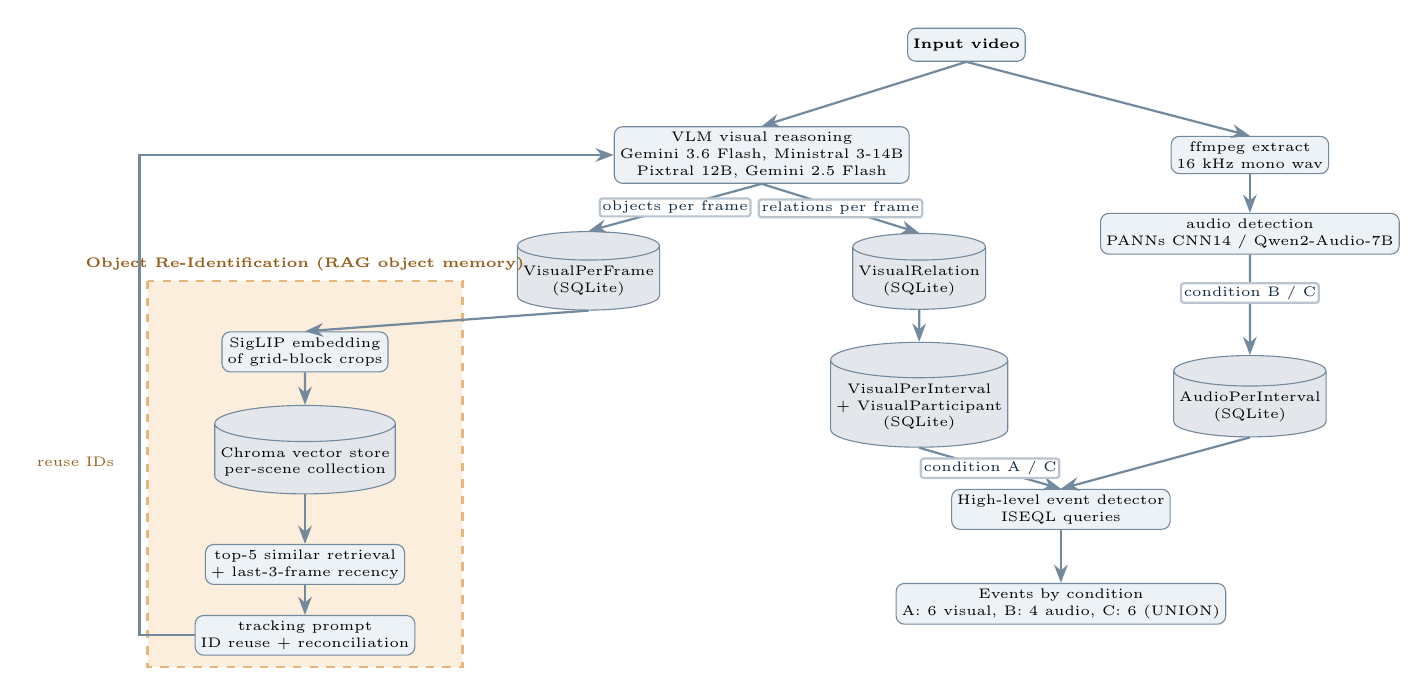
\begin{tikzpicture}[
  box/.style={rectangle,draw=navy!60,fill=navypale,rounded corners=3pt,align=center,minimum height=0.42cm,font=\tiny,inner sep=2pt},
  db/.style={cylinder,draw=navy!60,fill=navy!12,shape border rotate=90,aspect=0.2,minimum height=0.48cm,minimum width=1.55cm,align=center,font=\tiny,inner sep=2pt},
  arrow/.style={-Stealth,thick,navy!60},
  run/.style={font=\tiny,align=center,text=navy!70!black,fill=white,draw=navy!30,inner sep=1pt,rounded corners=1pt},
]
% INPUT + PERCEPTION
\node[box] (video) at (0.6,3.9) {\textbf{Input video}};
\node[box] (vlm) at (-2.0,2.5) {VLM visual reasoning\\Gemini 3.6 Flash, Ministral 3-14B\\Pixtral 12B, Gemini 2.5 Flash};
\node[box] (ff) at (4.2,2.5) {ffmpeg extract\\16 kHz mono wav};

% STORAGE LEVEL (database cylinders)
\node[db] (vpf) at (-4.2,0.9) {VisualPerFrame\\(SQLite)};
\node[db] (vrel) at (0.0,0.9) {VisualRelation\\(SQLite)};
\node[box] (aud) at (4.2,1.5) {audio detection\\PANNs CNN14 / Qwen2-Audio-7B};
\node[db] (aint) at (4.2,-0.7) {AudioPerInterval\\(SQLite)};

% INTERVALS + OUTPUT
\node[db] (vint) at (0.0,-0.7) {VisualPerInterval\\+ VisualParticipant\\(SQLite)};
\node[box] (det) at (1.8,-2.0) {High-level event detector\\ISEQL queries};
\node[box] (ev) at (1.8,-3.2) {Events by condition\\A: 6 visual, B: 4 audio, C: 6 (UNION)};

% RAG SUBTREE (wide shaded panel)
\fill[amberpale] (-9.8,0.9) rectangle (-5.8,-4.0);
\draw[amber!60,dashed,thick] (-9.8,0.9) rectangle (-5.8,-4.0);
\node[font=\tiny\bfseries,text=amber!70!black,anchor=south] at (-7.8,0.9) {Object Re-Identification (RAG object memory)};
\node[box] (sig) at (-7.8,0.0) {SigLIP embedding\\of grid-block crops};
\node[db] (chroma) at (-7.8,-1.4) {Chroma vector store\\per-scene collection};
\node[box] (retr) at (-7.8,-2.7) {top-5 similar retrieval\\+ last-3-frame recency};
\node[box] (track) at (-7.8,-3.6) {tracking prompt\\ID reuse + reconciliation};

% EDGES
\draw[arrow] (video.south) -- (vlm.north);
\draw[arrow] (video.south) -- (ff.north);
\draw[arrow] (vlm.south) -- (vpf.north) node[pos=0.5,run]{objects per frame};
\draw[arrow] (vlm.south) -- (vrel.north) node[pos=0.5,run]{relations per frame};
\draw[arrow] (ff.south) -- (aud.north);
\draw[arrow] (aud.south) -- (aint.north) node[midway,yshift=1.5mm,run]{condition B / C};
\draw[arrow] (vrel.south) -- (vint.north);
\draw[arrow] (vint.south) -- (det.north) node[midway,run]{condition A / C};
\draw[arrow] (aint.south) -- (det.north);
\draw[arrow] (det.south) -- (ev.north);
\draw[arrow] (vpf.south) -- (sig.north);
\draw[arrow] (sig.south) -- (chroma.north);
\draw[arrow] (chroma.south) -- (retr.north);
\draw[arrow] (retr.south) -- (track.north);
\draw[arrow] (track.west) -- ++(-0.7,0) |- (vlm.west);
\node[font=\tiny,text=amber!70!black,anchor=east] at (-10.1,-1.4) {reuse IDs};
\end{tikzpicture}}}
\end{frame}

% ── APPENDIX: DATABASE SCHEMA ──

% ── APPENDIX: DATABASE SCHEMA ──
\begingroup
\setlength{\fboxsep}{0.5pt}  % minimal padding so PK/FK boxes don't add row height
\begin{frame}{Appendix: Database Schema}
\centering
\makebox[\textwidth][c]{\resizebox{1.02\textwidth}{!}{%
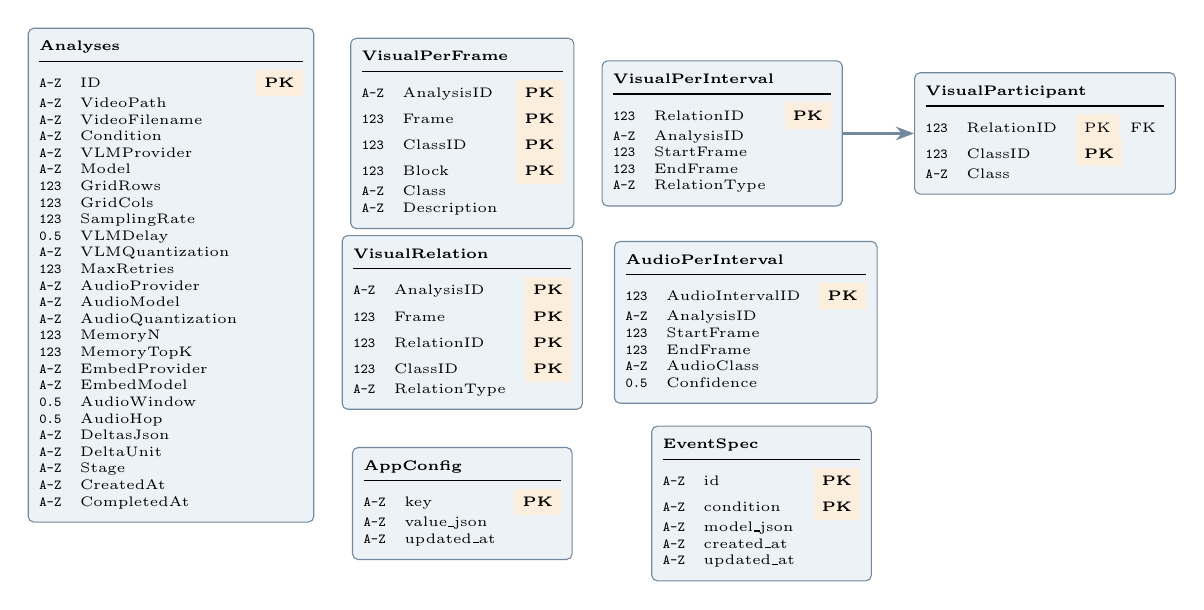
\begin{tikzpicture}[
  tbl/.style={rectangle,draw=navy!60,fill=navypale,rounded corners=2pt,align=left,inner sep=4pt,font=\tiny},
  arrow/.style={-Stealth,thick,navy!60},
  hd/.style={font=\tiny\bfseries,text=navy!70!black},
  run/.style={font=\tiny,text=navy!50!black,fill=white,draw=navy!30,inner sep=1pt,rounded corners=1pt},
]
% ANALYSES (tall, left column)
\node[tbl] (analyses) at (-5.3,0.4) {%
\begin{tabular}{@{}l@{\quad}l@{\quad}l@{}}
\multicolumn{3}{@{}l@{}}{\textbf{Analyses}}\\
\midrule
\strut \texttt{A-Z} & ID & \colorbox{amberpale}{\textbf{PK}}\\
\strut \texttt{A-Z} & VideoPath & \\
\strut \texttt{A-Z} & VideoFilename & \\
\strut \texttt{A-Z} & Condition & \\
\strut \texttt{A-Z} & VLMProvider & \\
\strut \texttt{A-Z} & Model & \\
\strut \texttt{123} & GridRows & \\
\strut \texttt{123} & GridCols & \\
\strut \texttt{123} & SamplingRate & \\
\strut \texttt{0.5} & VLMDelay & \\
\strut \texttt{A-Z} & VLMQuantization & \\
\strut \texttt{123} & MaxRetries & \\
\strut \texttt{A-Z} & AudioProvider & \\
\strut \texttt{A-Z} & AudioModel & \\
\strut \texttt{A-Z} & AudioQuantization & \\
\strut \texttt{123} & MemoryN & \\
\strut \texttt{123} & MemoryTopK & \\
\strut \texttt{A-Z} & EmbedProvider & \\
\strut \texttt{A-Z} & EmbedModel & \\
\strut \texttt{0.5} & AudioWindow & \\
\strut \texttt{0.5} & AudioHop & \\
\strut \texttt{A-Z} & DeltasJson & \\
\strut \texttt{A-Z} & DeltaUnit & \\
\strut \texttt{A-Z} & Stage & \\
\strut \texttt{A-Z} & CreatedAt & \\
\strut \texttt{A-Z} & CompletedAt & \\
\end{tabular}};

% TOP ROW
\node[tbl] (vpf) at (-1.6,2.2) {%
\begin{tabular}{@{}l@{\quad}l@{\quad}l@{}}
\multicolumn{3}{@{}l@{}}{\textbf{VisualPerFrame}}\\
\midrule
\strut \texttt{A-Z} & AnalysisID & \colorbox{amberpale}{\textbf{PK}}\\
\strut \texttt{123} & Frame & \colorbox{amberpale}{\textbf{PK}}\\
\strut \texttt{123} & ClassID & \colorbox{amberpale}{\textbf{PK}}\\
\strut \texttt{123} & Block & \colorbox{amberpale}{\textbf{PK}}\\
\strut \texttt{A-Z} & Class & \\
\strut \texttt{A-Z} & Description & \\
\end{tabular}};
\node[tbl] (vint) at (1.7,2.2) {%
\begin{tabular}{@{}l@{\quad}l@{\quad}l@{}}
\multicolumn{3}{@{}l@{}}{\textbf{VisualPerInterval}}\\
\midrule
\strut \texttt{123} & RelationID & \colorbox{amberpale}{\textbf{PK}}\\
\strut \texttt{A-Z} & AnalysisID & \\
\strut \texttt{123} & StartFrame & \\
\strut \texttt{123} & EndFrame & \\
\strut \texttt{A-Z} & RelationType & \\
\end{tabular}};
\node[tbl] (vpart) at (5.8,2.2) {%
\begin{tabular}{@{}l@{\quad}l@{\quad}l@{}}
\multicolumn{3}{@{}l@{}}{\textbf{VisualParticipant}}\\
\midrule
\strut \texttt{123} & RelationID & \colorbox{amberpale}{PK}\hspace{1pt}\colorbox{navypale}{FK}\\
\strut \texttt{123} & ClassID & \colorbox{amberpale}{\textbf{PK}}\\
\strut \texttt{A-Z} & Class & \\
\end{tabular}};

% MIDDLE ROW
\node[tbl] (vrel) at (-1.6,-0.2) {%
\begin{tabular}{@{}l@{\quad}l@{\quad}l@{}}
\multicolumn{3}{@{}l@{}}{\textbf{VisualRelation}}\\
\midrule
\strut \texttt{A-Z} & AnalysisID & \colorbox{amberpale}{\textbf{PK}}\\
\strut \texttt{123} & Frame & \colorbox{amberpale}{\textbf{PK}}\\
\strut \texttt{123} & RelationID & \colorbox{amberpale}{\textbf{PK}}\\
\strut \texttt{123} & ClassID & \colorbox{amberpale}{\textbf{PK}}\\
\strut \texttt{A-Z} & RelationType & \\
\end{tabular}};
\node[tbl] (aint) at (2.0,-0.2) {%
\begin{tabular}{@{}l@{\quad}l@{\quad}l@{}}
\multicolumn{3}{@{}l@{}}{\textbf{AudioPerInterval}}\\
\midrule
\strut \texttt{123} & AudioIntervalID & \colorbox{amberpale}{\textbf{PK}}\\
\strut \texttt{A-Z} & AnalysisID & \\
\strut \texttt{123} & StartFrame & \\
\strut \texttt{123} & EndFrame & \\
\strut \texttt{A-Z} & AudioClass & \\
\strut \texttt{0.5} & Confidence & \\
\end{tabular}};

% BOTTOM ROW
\node[tbl] (config) at (-1.6,-2.5) {%
\begin{tabular}{@{}l@{\quad}l@{\quad}l@{}}
\multicolumn{3}{@{}l@{}}{\textbf{AppConfig}}\\
\midrule
\strut \texttt{A-Z} & key & \colorbox{amberpale}{\textbf{PK}}\\
\strut \texttt{A-Z} & value\_json & \\
\strut \texttt{A-Z} & updated\_at & \\
\end{tabular}};
\node[tbl] (espec) at (2.2,-2.5) {%
\begin{tabular}{@{}l@{\quad}l@{\quad}l@{}}
\multicolumn{3}{@{}l@{}}{\textbf{EventSpec}}\\
\midrule
\strut \texttt{A-Z} & id & \colorbox{amberpale}{\textbf{PK}}\\
\strut \texttt{A-Z} & condition & \colorbox{amberpale}{\textbf{PK}}\\
\strut \texttt{A-Z} & model\_json & \\
\strut \texttt{A-Z} & created\_at & \\
\strut \texttt{A-Z} & updated\_at & \\
\end{tabular}};

% FOREIGN KEY (only declared FK in the schema)
\draw[arrow] (vint.east) -- (vpart.west);\end{tikzpicture}}}
\end{frame}
\endgroup

\begin{frame}{Appendix: Complete Multimodal Ablation (Condition C), Rows 1-16}
\centering
\footnotesize
\vspace{\baselineskip}
\resizebox{\textwidth}{!}{%
\begin{tabular}{lcccccccc}
\toprule
VLM + Audio Model & Window (s) & Hop (s) & F1 & Precision & Recall & TP & FP & FN \\
\midrule
    \textbf{Gemini 3.6 Flash + Qwen2-Audio} & \textbf{5.0} & \textbf{2.5} & \textbf{0.938} & \textbf{0.882} & \textbf{1.000} & \textbf{30} & \textbf{4} & \textbf{0} \\
    Gemini 3.6 Flash + Qwen2-Audio & 2.5 & 1.25 & 0.923 & 0.857 & 1.000 & 30 & 5 & 0 \\
    Gemini 3.6 Flash + Qwen2-Audio & 5.0 & 5.0 & 0.903 & 0.875 & 0.933 & 28 & 4 & 2 \\
    Gemini 3.6 Flash + PANNs CNN14 & 5.0 & 5.0 & 0.903 & 0.875 & 0.933 & 28 & 4 & 2 \\
    Gemini 3.6 Flash + PANNs CNN14 & 10.0 & 10.0 & 0.903 & 0.875 & 0.933 & 28 & 4 & 2 \\
    Gemini 3.6 Flash + PANNs CNN14 & 10.0 & 5.0 & 0.903 & 0.875 & 0.933 & 28 & 4 & 2 \\
    Gemini 3.6 Flash + Qwen2-Audio & 10.0 & 10.0 & 0.889 & 0.848 & 0.933 & 28 & 5 & 2 \\
    Gemini 3.6 Flash + Qwen2-Audio & 10.0 & 5.0 & 0.889 & 0.848 & 0.933 & 28 & 5 & 2 \\
    Gemini 3.6 Flash + PANNs CNN14 & 1.0 & 1.0 & 0.889 & 0.848 & 0.933 & 28 & 5 & 2 \\
    Gemini 3.6 Flash + PANNs CNN14 & 1.0 & 0.50 & 0.889 & 0.848 & 0.933 & 28 & 5 & 2 \\
    Gemini 3.6 Flash + PANNs CNN14 & 2.5 & 2.5 & 0.875 & 0.824 & 0.933 & 28 & 6 & 2 \\
    Gemini 3.6 Flash + PANNs CNN14 & 2.5 & 1.25 & 0.875 & 0.824 & 0.933 & 28 & 6 & 2 \\
    Gemini 3.6 Flash + PANNs CNN14 & 5.0 & 2.5 & 0.875 & 0.824 & 0.933 & 28 & 6 & 2 \\
    Gemini 3.6 Flash + Qwen2-Audio & 2.5 & 2.5 & 0.857 & 0.818 & 0.900 & 27 & 6 & 3 \\
    Ministral 3-14B + Qwen2-Audio & 5.0 & 2.5 & 0.825 & 0.788 & 0.867 & 26 & 7 & 4 \\
    Gemini 2.5 Flash + Qwen2-Audio & 5.0 & 2.5 & 0.820 & 0.806 & 0.833 & 25 & 6 & 5 \\
\bottomrule
\end{tabular}}
\end{frame}

\begin{frame}{Appendix: Complete Multimodal Ablation (Condition C), Rows 17-32}
\centering
\footnotesize
\vspace{\baselineskip}
\resizebox{\textwidth}{!}{%
\begin{tabular}{lcccccccc}
\toprule
VLM + Audio Model & Window (s) & Hop (s) & F1 & Precision & Recall & TP & FP & FN \\
\midrule
    Ministral 3-14B + Qwen2-Audio & 2.5 & 1.25 & 0.812 & 0.765 & 0.867 & 26 & 8 & 4 \\
    Gemini 2.5 Flash + Qwen2-Audio & 2.5 & 1.25 & 0.806 & 0.781 & 0.833 & 25 & 7 & 5 \\
    Pixtral 12B + Qwen2-Audio & 5.0 & 2.5 & 0.794 & 0.758 & 0.833 & 25 & 8 & 5 \\
    Pixtral 12B + Qwen2-Audio & 2.5 & 1.25 & 0.781 & 0.735 & 0.833 & 25 & 9 & 5 \\
    Ministral 3-14B + Qwen2-Audio & 5.0 & 5.0 & 0.767 & 0.767 & 0.767 & 23 & 7 & 7 \\
    Ministral 3-14B + Qwen2-Audio & 10.0 & 10.0 & 0.767 & 0.767 & 0.767 & 23 & 7 & 7 \\
    Ministral 3-14B + Qwen2-Audio & 10.0 & 5.0 & 0.767 & 0.767 & 0.767 & 23 & 7 & 7 \\
    Ministral 3-14B + PANNs CNN14 & 5.0 & 5.0 & 0.767 & 0.767 & 0.767 & 23 & 7 & 7 \\
    Ministral 3-14B + PANNs CNN14 & 10.0 & 10.0 & 0.767 & 0.767 & 0.767 & 23 & 7 & 7 \\
    Ministral 3-14B + PANNs CNN14 & 10.0 & 5.0 & 0.767 & 0.767 & 0.767 & 23 & 7 & 7 \\
    Gemini 2.5 Flash + Qwen2-Audio & 5.0 & 5.0 & 0.759 & 0.786 & 0.733 & 22 & 6 & 8 \\
    Gemini 2.5 Flash + PANNs CNN14 & 5.0 & 5.0 & 0.759 & 0.786 & 0.733 & 22 & 6 & 8 \\
    Gemini 2.5 Flash + PANNs CNN14 & 10.0 & 10.0 & 0.759 & 0.786 & 0.733 & 22 & 6 & 8 \\
    Gemini 2.5 Flash + PANNs CNN14 & 10.0 & 5.0 & 0.759 & 0.786 & 0.733 & 22 & 6 & 8 \\
    Ministral 3-14B + PANNs CNN14 & 1.0 & 1.0 & 0.754 & 0.742 & 0.767 & 23 & 8 & 7 \\
    Ministral 3-14B + PANNs CNN14 & 1.0 & 0.50 & 0.754 & 0.742 & 0.767 & 23 & 8 & 7 \\
\bottomrule
\end{tabular}}
\end{frame}

\begin{frame}{Appendix: Complete Multimodal Ablation (Condition C), Rows 33-48}
\centering
\footnotesize
\vspace{\baselineskip}
\resizebox{\textwidth}{!}{%
\begin{tabular}{lcccccccc}
\toprule
VLM + Audio Model & Window (s) & Hop (s) & F1 & Precision & Recall & TP & FP & FN \\
\midrule
    Ministral 3-14B + PANNs CNN14 & 2.5 & 2.5 & 0.754 & 0.742 & 0.767 & 23 & 8 & 7 \\
    Ministral 3-14B + PANNs CNN14 & 2.5 & 1.25 & 0.754 & 0.742 & 0.767 & 23 & 8 & 7 \\
    Gemini 3.6 Flash + Qwen2-Audio & 1.0 & 0.50 & 0.747 & 0.622 & 0.933 & 28 & 17 & 2 \\
    Gemini 2.5 Flash + Qwen2-Audio & 10.0 & 10.0 & 0.746 & 0.759 & 0.733 & 22 & 7 & 8 \\
    Gemini 2.5 Flash + Qwen2-Audio & 10.0 & 5.0 & 0.746 & 0.759 & 0.733 & 22 & 7 & 8 \\
    Gemini 2.5 Flash + PANNs CNN14 & 1.0 & 1.0 & 0.746 & 0.759 & 0.733 & 22 & 7 & 8 \\
    Gemini 2.5 Flash + PANNs CNN14 & 1.0 & 0.50 & 0.746 & 0.759 & 0.733 & 22 & 7 & 8 \\
    Ministral 3-14B + PANNs CNN14 & 5.0 & 2.5 & 0.742 & 0.719 & 0.767 & 23 & 9 & 7 \\
    Gemini 2.5 Flash + PANNs CNN14 & 2.5 & 2.5 & 0.733 & 0.733 & 0.733 & 22 & 8 & 8 \\
    Gemini 2.5 Flash + PANNs CNN14 & 2.5 & 1.25 & 0.733 & 0.733 & 0.733 & 22 & 8 & 8 \\
    Gemini 2.5 Flash + PANNs CNN14 & 5.0 & 2.5 & 0.733 & 0.733 & 0.733 & 22 & 8 & 8 \\
    Gemini 3.6 Flash + Qwen2-Audio & 1.0 & 1.0 & 0.727 & 0.596 & 0.933 & 28 & 19 & 2 \\
    Ministral 3-14B + Qwen2-Audio & 2.5 & 2.5 & 0.721 & 0.710 & 0.733 & 22 & 9 & 8 \\
    Gemini 2.5 Flash + Qwen2-Audio & 2.5 & 2.5 & 0.712 & 0.724 & 0.700 & 21 & 8 & 9 \\
    Pixtral 12B + Qwen2-Audio & 5.0 & 5.0 & 0.712 & 0.724 & 0.700 & 21 & 8 & 9 \\
    Pixtral 12B + PANNs CNN14 & 5.0 & 5.0 & 0.712 & 0.724 & 0.700 & 21 & 8 & 9 \\
\bottomrule
\end{tabular}}
\end{frame}

\begin{frame}{Appendix: Complete Multimodal Ablation (Condition C), Rows 49-64}
\centering
\footnotesize
\vspace{\baselineskip}
\resizebox{\textwidth}{!}{%
\begin{tabular}{lcccccccc}
\toprule
VLM + Audio Model & Window (s) & Hop (s) & F1 & Precision & Recall & TP & FP & FN \\
\midrule
    Pixtral 12B + PANNs CNN14 & 1.0 & 0.50 & 0.700 & 0.700 & 0.700 & 21 & 9 & 9 \\
    Pixtral 12B + PANNs CNN14 & 2.5 & 2.5 & 0.700 & 0.700 & 0.700 & 21 & 9 & 9 \\
    Pixtral 12B + PANNs CNN14 & 2.5 & 1.25 & 0.700 & 0.700 & 0.700 & 21 & 9 & 9 \\
    Pixtral 12B + Qwen2-Audio & 10.0 & 10.0 & 0.690 & 0.714 & 0.667 & 20 & 8 & 10 \\
    Pixtral 12B + Qwen2-Audio & 10.0 & 5.0 & 0.690 & 0.714 & 0.667 & 20 & 8 & 10 \\
    Pixtral 12B + PANNs CNN14 & 10.0 & 10.0 & 0.690 & 0.714 & 0.667 & 20 & 8 & 10 \\
    Pixtral 12B + PANNs CNN14 & 10.0 & 5.0 & 0.690 & 0.714 & 0.667 & 20 & 8 & 10 \\
    Pixtral 12B + PANNs CNN14 & 5.0 & 2.5 & 0.689 & 0.677 & 0.700 & 21 & 10 & 9 \\
    Pixtral 12B + PANNs CNN14 & 1.0 & 1.0 & 0.678 & 0.690 & 0.667 & 20 & 9 & 10 \\
    Pixtral 12B + Qwen2-Audio & 2.5 & 2.5 & 0.667 & 0.667 & 0.667 & 20 & 10 & 10 \\
    Ministral 3-14B + Qwen2-Audio & 1.0 & 0.50 & 0.639 & 0.548 & 0.767 & 23 & 19 & 7 \\
    Gemini 2.5 Flash + Qwen2-Audio & 1.0 & 0.50 & 0.639 & 0.548 & 0.767 & 23 & 19 & 7 \\
    Ministral 3-14B + Qwen2-Audio & 1.0 & 1.0 & 0.622 & 0.523 & 0.767 & 23 & 21 & 7 \\
    Pixtral 12B + Qwen2-Audio & 1.0 & 0.50 & 0.611 & 0.524 & 0.733 & 22 & 20 & 8 \\
    Gemini 2.5 Flash + Qwen2-Audio & 1.0 & 1.0 & 0.603 & 0.512 & 0.733 & 22 & 21 & 8 \\
    Pixtral 12B + Qwen2-Audio & 1.0 & 1.0 & 0.575 & 0.488 & 0.700 & 21 & 22 & 9 \\
\bottomrule
\end{tabular}}
\end{frame}


% ── BIBLIOGRAPHY ──
\begin{frame}{References}
\footnotesize
\begin{itemize}
\setlength{\itemsep}{0.3em}

\item S.~Helmer and F.~Persia. High-level Surveillance Event Detection Using an Interval-based Query Language. In \emph{Proc.\ ICSC}, pp.\ 39--46. IEEE, 2016.

\item F.~Persia, F.~Bettini, and S.~Helmer. An Interactive Framework for Video Surveillance Event Detection and Modeling. In \emph{Proc.\ CIKM}, pp.\ 2515--2518. ACM, 2017.

\item F.~Persia et al. Modeling and detecting high-level events in healthcare applications exploiting ISEQL+. \emph{Soft Computing}, 30(5):3667--3690, 2026.

\item X.~Zhai, B.~Mustafa, A.~Kolesnikov, and L.~Beyer. Sigmoid Loss for Language Image Pre-Training (SigLIP). \emph{Proc.\ ICCV}, pp.\ 11975--11986, 2023.

\item Q.~Kong et al. {PANNs}: Large-Scale Pretrained Audio Neural Networks for Audio Pattern Recognition. \emph{IEEE/ACM Trans.\ Audio, Speech, Lang.\ Process.}, 28:2880--2894, 2020.

\item Y.~Chu et al. Qwen2-Audio Technical Report. \emph{arXiv preprint arXiv:2407.10759}, 2024.

\item V.~Crescitelli et al. {VIS MODE}: Complex Event Detection from VLM-Based Video Observations. In \emph{Proc.\ ECCV (Demo Track)}. 2026.

\end{itemize}
\end{frame}

\end{document}
